

\section{OpticalElement: \textquotedbl{}ELT\textquotedbl{}%
  \label{opticalelement-elt}%
}

\textbf{Element}: telescope

\textbf{Alias}: TEL

\textbf{Description}: The extremely large telescope


\subsection{Global properties%
  \label{global-properties}%
}

\begin{quote}
\begin{alltt}
\begin{lstlisting}[frame=single]
 temperature : !ATMO.temperature
element_name : ELT
\end{lstlisting}
\end{alltt}
\end{quote}


\subsection{Effects%
  \label{effects}%
}

Summary of Effects included in this optical element:

\setlength{\DUtablewidth}{\linewidth}
\begin{longtable*}[c]{|p{0.098\DUtablewidth}|p{0.284\DUtablewidth}|p{0.145\DUtablewidth}|p{0.110\DUtablewidth}|p{0.179\DUtablewidth}|}
\hline
\textbf{%
element
} & \textbf{%
name
} & \textbf{%
class
} & \textbf{%
included
} & \textbf{%
z\_orders
} \\
\hline
\endfirsthead
\hline
\textbf{%
element
} & \textbf{%
name
} & \textbf{%
class
} & \textbf{%
included
} & \textbf{%
z\_orders
} \\
\hline
\endhead
\multicolumn{5}{c}{\hfill ... continued on next page} \\
\endfoot
\endlastfoot

ELT
 & 
scope\_surface\_list
 & 
SurfaceList
 & 
True
 & 
{[}20, 120, 520{]}
 \\
\hline

ELT
 & 
scope\_vibration
 & 
Vibration
 & 
True
 & 
{[}244, 744{]}
 \\
\hline

ELT
 & 
eso\_combined\_reflection
 & 
TERCurve
 & 
False
 & 
{[}10, 110, 510{]}
 \\
\hline
\end{longtable*}
\label{tbl-elt}


\subsubsection{SurfaceList: \textquotedbl{}scope\_surface\_list\textquotedbl{}%
  \label{surfacelist-scope-surface-list}%
}

\textbf{Included by default}: \texttt{True}

\textbf{File Description}: list of ELT surfaces

\textbf{Class Description}: <no docstring>

\textbf{Changes}:

\begin{itemize}
\item 2018-11-19 (KL) Added meta data, added Action column

\item 2019-01-28 (KL) Fixed YAML format in meta data

\item 2020-08-17 (KL) Updated M1 and M4 dimensions according to ESO-253082\_4 sect 4.7 \textquotedbl{}all-glass\textquotedbl{} diameter

\item 2020-08-17 (KL) Pegged temperature to the atmosphere
\end{itemize}


\paragraph{Data%
  \label{data}%
}

\begin{figure}[H]
\noindent\makebox[\linewidth][c]{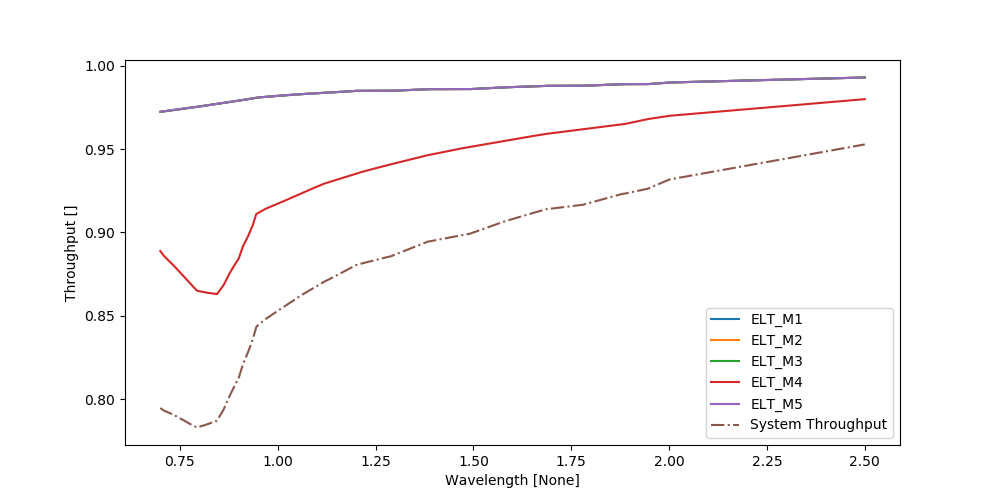
\includegraphics{scope_surface_list.png}}\phantomsection\label{fig-scope-surface-list}
\end{figure}

\setlength{\DUtablewidth}{\linewidth}
\begin{longtable*}[c]{|p{0.083\DUtablewidth}|p{0.072\DUtablewidth}|p{0.072\DUtablewidth}|p{0.072\DUtablewidth}|p{0.207\DUtablewidth}|p{0.128\DUtablewidth}|p{0.330\DUtablewidth}|}
\hline
\textbf{%
name
} & \textbf{%
outer
} & \textbf{%
inner
} & \textbf{%
angle
} & \textbf{%
temperature
} & \textbf{%
action
} & \textbf{%
filename
} \\
\hline
\endfirsthead
\hline
\textbf{%
name
} & \textbf{%
outer
} & \textbf{%
inner
} & \textbf{%
angle
} & \textbf{%
temperature
} & \textbf{%
action
} & \textbf{%
filename
} \\
\hline
\endhead
\multicolumn{7}{c}{\hfill ... continued on next page} \\
\endfoot
\endlastfoot

ELT\_M1
 & 
36.9
 & 
10.95
 & 
0.0
 & 
!ATMO.temperature
 & 
reflection
 & 
TER\_ELT\_mirror\_mgf2agal.dat
 \\
\hline

ELT\_M2
 & 
4.2
 & 
0.545
 & 
0.0
 & 
!ATMO.temperature
 & 
reflection
 & 
TER\_ELT\_mirror\_mgf2agal.dat
 \\
\hline

ELT\_M3
 & 
3.8
 & 
0.14
 & 
0.0
 & 
!ATMO.temperature
 & 
reflection
 & 
TER\_ELT\_mirror\_mgf2agal.dat
 \\
\hline

ELT\_M4
 & 
2.54
 & 
0.536
 & 
7.75
 & 
!ATMO.temperature
 & 
reflection
 & 
TER\_ELT\_mirror\_aluminium.dat
 \\
\hline

ELT\_M5
 & 
2.66
 & 
0.0
 & 
37.25
 & 
!ATMO.temperature
 & 
reflection
 & 
TER\_ELT\_mirror\_mgf2agal.dat
 \\
\hline
\end{longtable*}
\label{tbl-scope-surface-list}


\paragraph{Meta-data%
  \label{meta-data}%
}

\begin{quote}
\begin{alltt}
\begin{lstlisting}[frame=single]
            filename : LIST_mirrors_ELT.tbl
                name : scope_surface_list
         temperature : !ATMO.temperature
        element_name : ELT
              author : Oliver Czoske, Kieran Leschinski
              source : ESO ELT DRM, ESO-253082_4
        date_created : 2018-11-19
       date_modified : 2020-08-17
              status : Design, pre MICADO-FDR mirror list
          outer_unit : m
          inner_unit : m
          angle_unit : degree
    temperature_unit : deg_C
               notes : ['2020-08-17 (KL) Coatings match those described in ESO-253082_4']
             z_order : [20, 120, 520]
             include : True
        ignore_wings : False
            wave_min : !SIM.spectral.wave_min
            wave_max : !SIM.spectral.wave_max
           wave_unit : !SIM.spectral.wave_unit
            wave_bin : !SIM.spectral.spectral_resolution
 report_plot_include : True
report_table_include : True
  minimum_throughput : !SIM.spectral.minimum_throughput
             etendue : !TEL.etendue
\end{lstlisting}
\end{alltt}
\end{quote}


\subsubsection{Vibration: \textquotedbl{}scope\_vibration\textquotedbl{}%
  \label{vibration-scope-vibration}%
}

\textbf{Included by default}: \texttt{True}

\textbf{File Description}: residual vibration of telescope

\textbf{Class Description}: Creates a wavelength independent kernel image

\textbf{Changes}:

\begin{itemize}
\item \end{itemize}


\paragraph{Data%
  \label{id1}%
}

\begin{figure}[H]
\noindent\makebox[\linewidth][c]{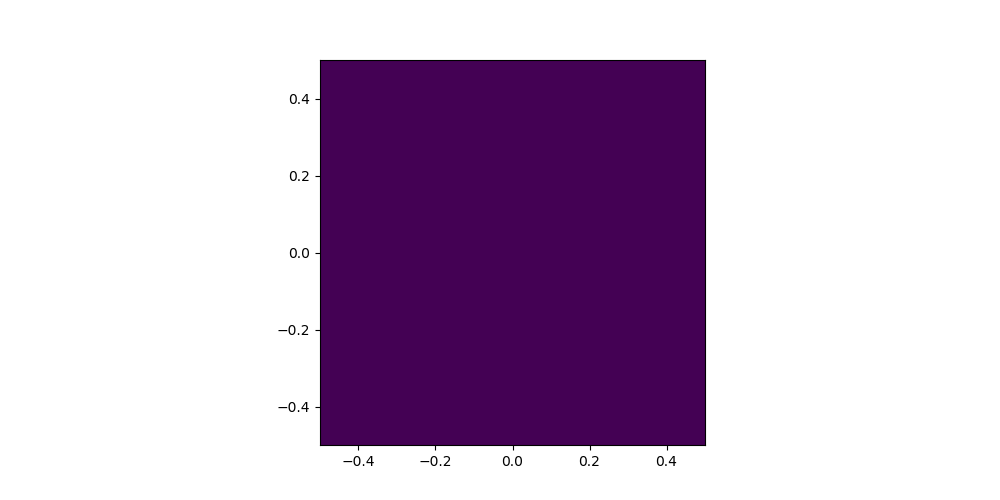
\includegraphics{scope_vibration.png}}\phantomsection\label{fig-scope-vibration}
\end{figure}


\paragraph{Meta-data%
  \label{id2}%
}

\begin{quote}
\begin{alltt}
\begin{lstlisting}[frame=single]
            filename : None
                name : scope_vibration
         temperature : 7
        element_name : ELT
                fwhm : 0.001
         pixel_scale : 0.004
             z_order : [244, 744]
             include : True
       flux_accuracy : 0.001
      sub_pixel_flag : False
       convolve_mode : full
            wave_key : WAVE0
    normalise_kernel : True
 report_plot_include : True
report_table_include : False
       width_n_fwhms : 4
\end{lstlisting}
\end{alltt}
\end{quote}


\subsubsection{TERCurve: \textquotedbl{}eso\_combined\_reflection\textquotedbl{}%
  \label{tercurve-eso-combined-reflection}%
}

\textbf{Included by default}: \texttt{False}

\textbf{File Description}: single combined reflection curve for clean ELT 5 mirror combination

\textbf{Class Description}: Transmission, Emissivity, Reflection Curve

\textbf{Changes}:

\begin{itemize}
\item 2019-11-06 (KL) Converted from .xlsx to .dat file, added ScopeSim meta data

\item 2020-07-09 (KL) Added inner and outer dimensions to meta, for use with MICADO-Sci

\item 2020-08-17 (KL) Added emissivity column according to ESO-253082\_4, sect 4.12.2
\end{itemize}


\paragraph{Data%
  \label{id3}%
}

\begin{figure}[H]
\noindent\makebox[\linewidth][c]{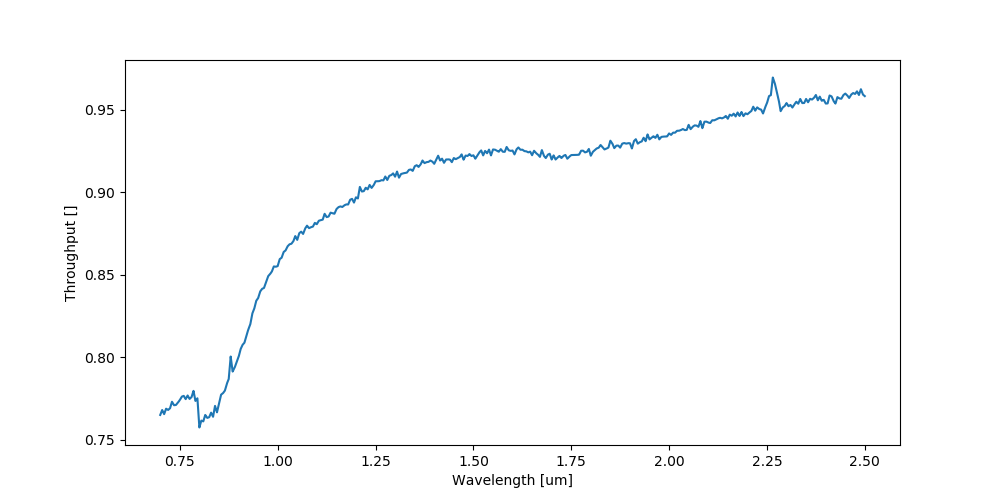
\includegraphics{eso_combined_reflection.png}}\phantomsection\label{fig-eso-combined-reflection}
\end{figure}


\paragraph{Meta-data%
  \label{id4}%
}

\begin{quote}
\begin{alltt}
\begin{lstlisting}[frame=single]
            filename : TER_ELT_system_20190611.dat
                name : eso_combined_reflection
             include : False
         temperature : 7
        element_name : ELT
          temperture : 7
              author : R. Holzloehner
              source : See ESO-306070 and ESO-293390 for background.
        date_created : 2018-09-18
       date_modified : 2019-06-11
                type : TERCurve
              status : design
              action : reflection
               outer : 37.3
          outer_unit : m
               inner : 11.1
          inner_unit : m
     wavelength_unit : um
               notes : ['Baseline coatings.', 'Fresh coatings without contamination.', '4nm roughness modeled.', 'Partly based on measured data by Tom Schneider (Gemini).', 'Reflection is for the combined M1-M5 system, not for individual mirrors', 'Emissivity is calculated from ESO-253082_4, sect 4.12.2']
             z_order : [10, 110, 510]
        ignore_wings : False
            wave_min : 0.7
            wave_max : 2.5
           wave_unit : um
            wave_bin : 0.0001
 report_plot_include : True
report_table_include : False
\end{lstlisting}
\end{alltt}
\end{quote}
